\documentclass[tikz,border=6pt]{standalone}
\usepackage[T1]{fontenc}
\usepackage[utf8]{inputenc}
\usepackage{pgfplots}
\usepgfplotslibrary{groupplots}
\usetikzlibrary{calc}
\pgfplotsset{compat=1.18}
\begin{document}
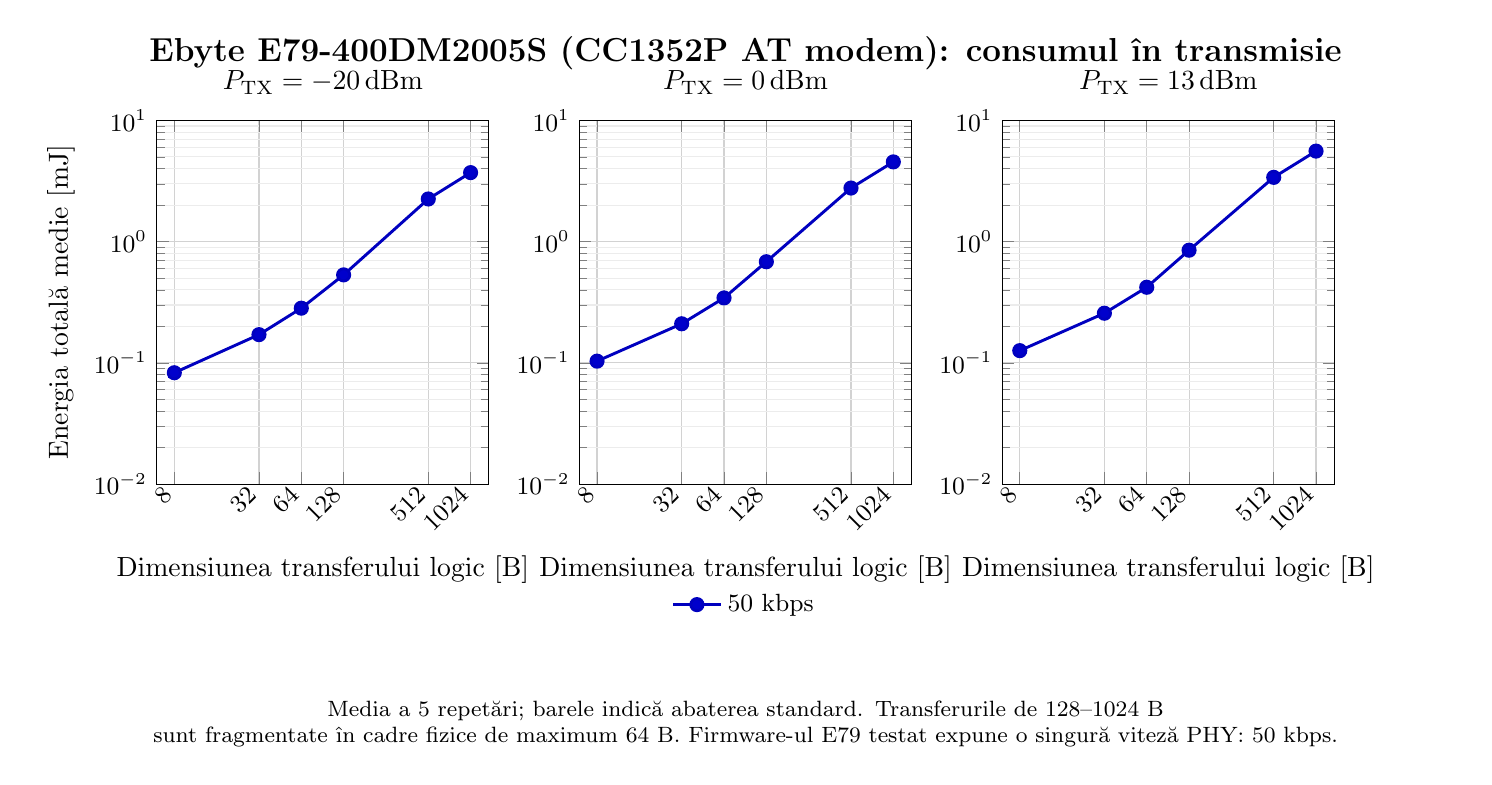
\begin{tikzpicture}
\begin{groupplot}[/pgf/number format/use comma,
  group style={group size=3 by 1, horizontal sep=1.15cm},
  width=5.8cm, height=6.2cm,
  xmode=log, log basis x={2}, ymode=log, log basis y={10},
  ymin=0.01, ymax=10,
  xmin=6, xmax=1382.4,
  xtick={8,32,64,128,512,1024}, xticklabels={8,32,64,128,512,1024},
  x tick label style={rotate=45, anchor=east, font=\small},
  y tick label style={font=\small},
  grid=both, minor grid style={gray!15}, major grid style={gray!35},
  xlabel={Dimensiunea transferului logic [B]},
  every axis plot/.append style={line width=1.05pt},
  error bars/error bar style={line width=0.35pt},
  legend style={font=\small, draw=none, fill=none,
    at={(0.5,-0.27)}, anchor=north, legend columns=2},
]
\nextgroupplot[title={\(P_{\mathrm{TX}}=-20\,\mathrm{dBm}\)}, ylabel={Energia totală medie [mJ]}]
\addplot+[blue!75!black, solid, mark=*, mark size=2.2pt,
  error bars/.cd, y dir=both, y explicit,
] coordinates {
  (8,0.0829053658) +- (0,0.00770405044)
  (32,0.170909392) +- (0,0.00295902953)
  (64,0.28257302) +- (0,0.00316853723)
  (128,0.532030854) +- (0,0.0350689458)
  (512,2.24904683) +- (0,0.0355941032)
  (1024,3.71091056) +- (0,0.0146927529)
};
\nextgroupplot[title={\(P_{\mathrm{TX}}=0\,\mathrm{dBm}\)}]
\addplot+[blue!75!black, solid, mark=*, mark size=2.2pt,
  error bars/.cd, y dir=both, y explicit,
] coordinates {
  (8,0.103319288) +- (0,0.00548363546)
  (32,0.210146884) +- (0,0.00218956303)
  (64,0.343410415) +- (0,0.0201956217)
  (128,0.682866098) +- (0,0.022084541)
  (512,2.76896971) +- (0,0.0323245624)
  (1024,4.5500768) +- (0,0.0140142201)
};
\addlegendentry{50 kbps}
\nextgroupplot[title={\(P_{\mathrm{TX}}=13\,\mathrm{dBm}\)}]
\addplot+[blue!75!black, solid, mark=*, mark size=2.2pt,
  error bars/.cd, y dir=both, y explicit,
] coordinates {
  (8,0.126110346) +- (0,0.0046818786)
  (32,0.256786687) +- (0,0.00404649346)
  (64,0.420437186) +- (0,0.0199228743)
  (128,0.849975348) +- (0,0.0200749542)
  (512,3.39264958) +- (0,0.035218882)
  (1024,5.58319835) +- (0,0.0162436864)
};
\end{groupplot}
\node[font=\bfseries\large] at ($(group c2r1.north)+(0,0.85cm)$)
  {Ebyte E79-400DM2005S (CC1352P AT modem): consumul în transmisie};
\node[font=\footnotesize, align=center, text width=18cm]
  at ($(group c2r1.south)+(0,-3.05cm)$)
  {Media a 5 repetări; barele indică abaterea standard. Transferurile de 128--1024 B\\
   sunt fragmentate în cadre fizice de maximum 64 B. Firmware-ul E79 testat expune o singură viteză PHY: 50 kbps.};
\end{tikzpicture}
\end{document}
